% Copyright 2004 by Till Tantau <tantau@users.sourceforge.net>.
%
% In principle, this file can be redistributed and/or modified under
% the terms of the GNU Public License, version 2.
%
% However, this file is supposed to be a template to be modified
% for your own needs. For this reason, if you use this file as a
% template and not specifically distribute it as part of a another
% package/program, I grant the extra permission to freely copy and
% modify this file as you see fit and even to delete this copyright
% notice. 

\documentclass[xcolor=table]{beamer}
\usepackage{menukeys}[os=win]
\usepackage{textcomp}
\usepackage{tcolorbox}
\usepackage{listings}
\lstset{
  basicstyle=\tiny\ttfamily,
}

% There are many different themes available for Beamer. A comprehensive
% list with examples is given here:
% http://deic.uab.es/~iblanes/beamer_gallery/index_by_theme.html
% You can uncomment the themes below if you would like to use a different
% one:
%\usetheme{AnnArbor}
%\usetheme{Antibes}
%\usetheme{Bergen}
%\usetheme{Berkeley}
%\usetheme{Berlin}
%\usetheme{Boadilla}
%\usetheme{boxes}
%\usetheme{CambridgeUS}
%\usetheme{Copenhagen}
%\usetheme{Darmstadt}
%\usetheme{default}
%\usetheme{Frankfurt}
%\usetheme{Goettingen}
%\usetheme{Hannover}
%\usetheme{Ilmenau}
\usetheme{JuanLesPins}
%\usetheme{Luebeck}
%\usetheme{Madrid}
%\usetheme{Malmoe}
%\usetheme{Marburg}
%\usetheme{Montpellier}
%\usetheme{PaloAlto}
%\usetheme{Pittsburgh}
%\usetheme{Rochester}
%\usetheme{Singapore}
%\usetheme{Szeged}
%\usetheme{Warsaw}
\setbeamerfont{block body}{size=\small}
\title{KF5004 - \texttt{NFS}}

% A subtitle is optional and this may be deleted
% \subtitle{(Using proximity detection)}

\author{Dr.~Neil~Eliot\inst{1} / Dr.~Alun~Moon\inst{1}}
% - Give the names in the same order as the appear in the paper.
% - Use the \inst{?} command only if the authors have different
%   affiliation.

%\renewcommand\appendixname{Appendix}

\institute[Northumbria University] % (optional, but mostly needed)
{
  \inst{1}
  Department of Computer and Information Sciences\\
  University of Northumbria
  % \and
  % \inst{2}
  % Department of Theoretical Philosophy\\
  % University of Elsewhere
}
% - Use the \inst command only if there are several affiliations.
% - Keep it simple, no one is interested in your street address.

\date{Session 9}
% - Either use conference name or its abbreviation.
% - Not really informative to the audience, more for people (including
%   yourself) who are reading the slides online

\subject{Introduction}
% This is only inserted into the PDF information catalog. Can be left
% out. 

% If you have a file called "university-logo-filename.xxx", where xxx
% is a graphic format that can be processed by latex or pdflatex,
% resp., then you can add a logo as follows:

% \pgfdeclareimage[height=0.5cm]{university-logo}{university-logo-filename}
% \logo{\pgfuseimage{university-logo}}

% Delete this, if you do not want the table of contents to pop up at
% the beginning of each subsection:
% \AtBeginSubsection[]
% {
%   \begin{frame}<beamer>{Outline}
%     \tableofcontents[currentsection,currentsubsection]
%   \end{frame}
% }

% Let's get started

\begin{document}

\begin{frame}
  \titlepage
\end{frame}

\begin{frame}{Introduction}
  \tableofcontents
  % You might wish to add the option [pausesections]
\end{frame}

% Section and subsections will appear in the presentation overview
% and table of contents.

\section{Introduction}
\subsection{Background}
\begin{frame}{Content Storage via \texttt{NFS}}
  \begin{itemize}
    \item Large scale web services require shared storage and a shared database.
    \item The database is used to store \texttt{Meta Data} and the Content Store to hold materials such as:-    
      \begin{itemize}
        \item Images
        \item Music
        \item Video
        \item Documents
      \end{itemize}
    \item The content store \textbf{should NOT} be used for application files (\texttt{PHP}) or \texttt{HTML} pages
      \begin{tcolorbox}
        \begin{center}
          \scriptsize Sometimes this cannot be voided due to the way an application has been developed. \\When developing applications take into consideration deployment!
        \end{center}
      \end{tcolorbox}
  \end{itemize}
\end{frame}

\begin{frame}{Full deployment (Where are we going with this?)}
  \begin{figure}
    \begin{center}
      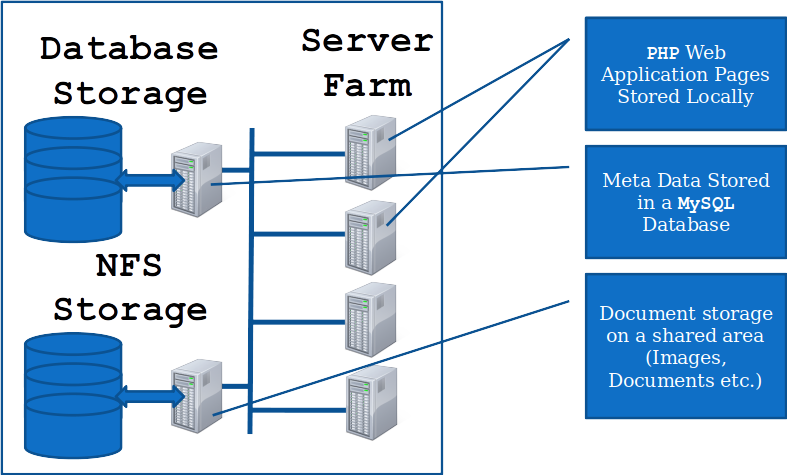
\includegraphics[width=1\linewidth]{FullDeployment.png}
    \end{center}
  \end{figure}
\end{frame}

\begin{frame}{\texttt{NFS} Security}
  \begin{itemize}
    \item Security is a big topic within \texttt{NFS}:
      \begin{itemize}
        \item Authentication infrastructures  
          \begin{itemize}
            \item \texttt{LDAP}
            \item \texttt{SMB}
            \item \texttt{rDNS} (\textbf{We will be covering this})
            \item \texttt{NFS} allows Unix environments to share \texttt{UID}s and \texttt{GID}s for authentication.
          \end{itemize}
      \end{itemize}
  \end{itemize}
  \begin{tcolorbox}
    \begin{center}
      \scriptsize Further details can be found at: \texttt{http://nfs.sourceforge.net/nfs-howto/ar01s06.html}
    \end{center}
  \end{tcolorbox}
\end{frame}

\begin{frame}{What is Content Storage?}
  \begin{figure}
    \begin{center}
      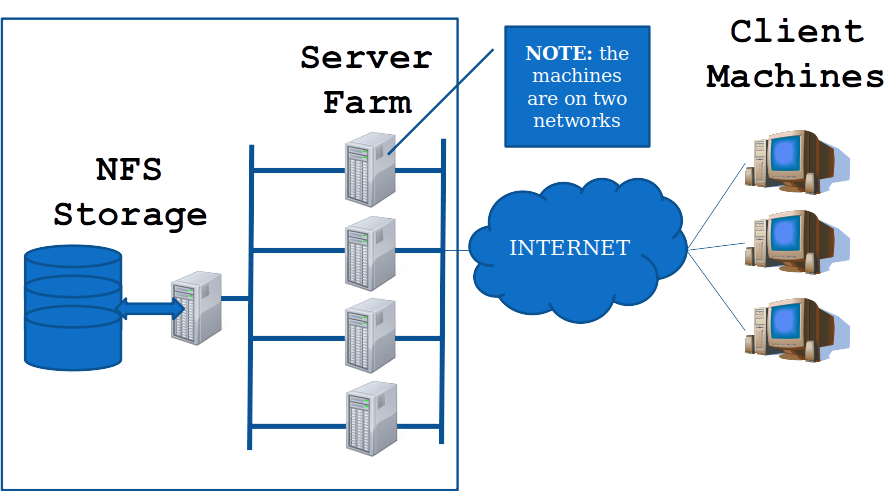
\includegraphics[width=1\linewidth]{WhatIs.png}
    \end{center}
  \end{figure}
\end{frame}

\section{Installation}
\subsection{\texttt{NFS} Server Installation}
\begin{frame}{\texttt{NFS} Installation}
  \begin{itemize}
    \item Like most services you need to install it from the \texttt{Ubuntu Repository}.
    \item You need to install the \texttt{NFS} Server Daemon.
      \begin{itemize}
        \item \texttt{\$sudo apt-get install nfs-kernel-server}
      \end{itemize}
  \end{itemize}
  \begin{tcolorbox}
    \begin{center}
      \scriptsize Have you updated your servers lately? (\texttt{update/upgrade}).
    \end{center}
  \end{tcolorbox}
\end{frame}

\begin{frame}[fragile]{\texttt{NFS} Installation}
  \begin{tcolorbox}
    \lstset{
      basicstyle=\tiny\ttfamily,
    }
    \begin{lstlisting}
Reading package lists... Done
Building dependency tree
Reading state information... Done
The following NEW packages will be installed:
  nfs-kernel-server
0 upgraded, 1 newly installed, 0 to remove and 23 not upgraded.
Need to get 0 B/124 kB of archives.
After this operation, 623 kB of additional disk space will be used.
Selecting previously deselected package nfs-kernel-server.
(Reading database ... 26245 files and directories currently installed.)
Unpacking nfs-kernel-server 
(from .../nfs-kernel-server_1%3a1.2.4-1ubuntu2_i386.deb) ...
Processing triggers for ureadahead ...
Processing triggers for man-db ...
Setting up nfs-kernel-server (1:1.2.4-1ubuntu2) ...
 * Stopping NFS kernel daemon                                 [ OK ]
 * Unexporting directories for NFS kernel daemon...           [ OK ]
 * Exporting directories for NFS kernel daemon...             [ OK ]              
exportfs: scandir /etc/exports.d: No such file or directory   [ OK ]
 * Starting NFS kernel daemon                                 [ OK ]
student@ubuntu:~$

    \end{lstlisting}
  \end{tcolorbox}
\end{frame}

\begin{frame}{\texttt{NFS} Configuration}
  \begin{itemize}
    \item \texttt{NFS} is configured through a configuration file.
    \item The \texttt{exports} file allows specific folders on the file system to be \textit{exposed} to the network infrastructure.
      \begin{itemize}
        \item \texttt{/etc/exports}
      \end{itemize}
  \end{itemize}
\end{frame}

\begin{frame}[fragile]{\texttt{NFS} Configuration - Public Access}
  \begin{itemize}
    \item The simplest way to export a folder is to export to any \texttt{NFS} client that wishes to attach.
      \begin{itemize}
        \item No security!
      \end{itemize}
    \item Edit the \texttt{/etc/exports} file and add directories (that exist). Using a * allows all clients to attach
  \end{itemize}
  \begin{tcolorbox}
    \lstset{
      basicstyle=\tiny\ttfamily,
    }
    \begin{lstlisting}
            /ubuntu	*(ro,sync,no_root_squash)
            /home 	*(rw,sync,no_root_squash)
    \end{lstlisting}
  \end{tcolorbox}
\end{frame}

\begin{frame}[fragile]{\texttt{NFS} Configuration - \texttt{rDNS} Authentication}
  \begin{itemize}
    \item Each line defines a directory and the hosts that are allowed to mount it. 
    \item A hostname can be a ``fully qualified'' or regular expressions can be used to define a name.
      \begin{itemize}
        \item i.e. Using the \texttt{*} and \texttt{?} wildcards allows fine grain control of multiple domain names.
      \end{itemize}
    \item e.g. \texttt{www*.student.co.uk} matches:
      \begin{itemize}
        \item \texttt{www1.student.co.uk}
        \item \texttt{www2.student.co.uk}
        \item \texttt{www32.student.co.uk}
      \end{itemize}
  \end{itemize}
  \begin{tcolorbox}
    \lstset{
      basicstyle=\tiny\ttfamily,
    }
    \begin{lstlisting}
      /ubuntu	www*.student.co.uk(ro,sync,no_root_squash)
      /home 	www*.student.co.uk(rw,sync,no_root_squash)
    \end{lstlisting}
  \end{tcolorbox}
\end{frame}

\begin{frame}{\texttt{NFS} Configuration - \texttt{rDNS} Authentication}
  \begin{itemize}
    \item Using a \texttt{URL} makes the \texttt{NFS} server use \texttt{rDNS} as an authentication protocol.
    \item The server uses the \texttt{IP} address of the connection to query the \texttt{DNS} Architecture for a hostname and validates the hostname against the entries.
  \end{itemize}
  \begin{tcolorbox}
    \begin{center}
      \scriptsize The \texttt{NFS} servers \texttt{IP} settings must be correctly configured for the reverse lookup to work.
    \end{center}
  \end{tcolorbox}
\end{frame}

\begin{frame}{\texttt{NFS} Configuration - \texttt{exports} file format}
  \begin{itemize}
    \item The hostname is followed by an optional comma-separated list of flags enclosed in parentheses. 
    \item Some of the values these flags may take are: 
      \begin{itemize}
        \item \texttt{secure} - This flag insists that requests be made from a reserved source port, i.e., one that is less than 1,024. This flag is set by default.
        \item \texttt{insecure} - This flag reverses the effect of the \texttt{secure} flag.
        \item \texttt{ro} - This flag causes the \texttt{NFS} mount to be read-only. This flag is enabled by default.
        \item \texttt{rw} - This option mounts file hierarchy read-write.
      \end{itemize}
      Continued....
  \end{itemize}
\end{frame}

\begin{frame}{\texttt{NFS} Configuration - \texttt{exports} file format}
  \begin{itemize}
    \item Flags:
      \begin{itemize}
        \item \texttt{root\_squash} - This security feature denies the superusers on the specified hosts any special access rights by mapping requests from \texttt{uid 0} on the client to the \texttt{uid 65534} (that is, -2) on the server. This \texttt{uid} should be associated with the \texttt{user nobody}.
        \item \texttt{no\_root\_squash} - Don't map requests from \texttt{uid 0}. This option is on by default, so superusers have superuser access to your system's exported directories.
      \end{itemize}
  \end{itemize}
  Continued....
\end{frame}

\begin{frame}{\texttt{NFS} Configuration - \texttt{exports} file format}
  \begin{itemize}
    \item Flags:
      \begin{itemize}
        \item \texttt{link\_relative} - This option converts absolute symbolic links (where the link contents start with a slash) into relative links. This option makes sense only when a host's entire filesystem is mounted; otherwise, some of the links might point to nowhere, or even worse, to files they were never meant to point to. This option is on by default.
        \item \texttt{link\_absolute} - This option leaves all symbolic links as they are (the normal behaviour for \texttt{NFS} servers).
      \end{itemize}
  \end{itemize}
  Continued....
\end{frame}

\begin{frame}{\texttt{NFS} Configuration - \texttt{exports} file format}
  \begin{itemize}
    \item Flags:
      \begin{itemize}
        \item \texttt{map\_identity} - This option tells the server to assume that the client uses the same \texttt{uid}s and \texttt{gid}s as the server. This option is on by default.
        \item \texttt{map\_daemon} - This option tells the \texttt{NFS} server to assume that client and server do not share the same \texttt{uid/gid} space. \texttt{rpc.nfsd} then builds a list that maps \texttt{ID}s between client and server by querying the client's \texttt{rpc.ugidd} daemon.
      \end{itemize}
  \end{itemize}
  Continued....
\end{frame}

\begin{frame}{\texttt{NFS} Configuration - \texttt{exports} file format}
  \begin{itemize}
    \item Flags:
      \begin{itemize}
        \item \texttt{map\_static} - This option allows you to specify the name of a file that contains a static map of \texttt{uid}s and \texttt{gid}s. For example, \texttt{map\_static=/etc/nfs/vlight.map} would specify the \texttt{/etc/nfs/vlight.map} file as a \texttt{uid/gid} map. 
        \item \texttt{ map\_nis} - This option causes the \texttt{NIS} server to do the \texttt{uid} and \texttt{gid} mapping.
        \item \texttt{anonuid} and \texttt{anongid} - These options allow you to specify the \texttt{uid} and \texttt{gid} of the anonymous account. This is useful if you have a volume exported for public mounts.
      \end{itemize}
  \end{itemize}
\end{frame}

\subsection{\texttt{NFS} Client Installation}
\begin{frame}{Background}
  \begin{itemize}
    \item A web server farm environment needs the \texttt{Apache} web servers to mount the \texttt{NFS} Server export to shared content.
  \end{itemize}
  \begin{tcolorbox}
      \noindent \scriptsize \textbf{REMEMBER:} You should \textbf{NOT} use this technique to ``common up'' the scripts as this will have an effect on performance and also system migrations.
      \begin{itemize}
        \item With the \texttt{PHP} files loaded locally to each server no network traffic is generated for page generation except meta data through database activity and shared content.
        \item You can upgrade servers in a sequence and test them as only one copy of the code exists.
      \end{itemize}
  \end{tcolorbox}
\end{frame}

\begin{frame}{\texttt{NFS} Client Installation}
  \begin{figure}
    \begin{center}
      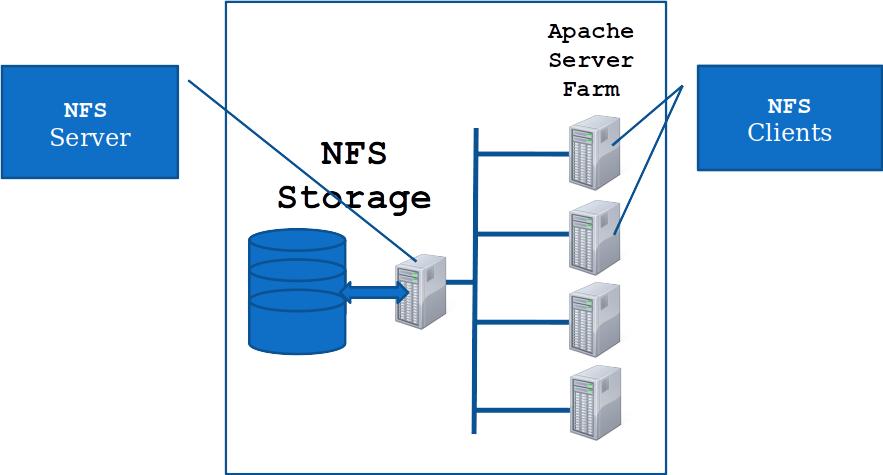
\includegraphics[width=1\linewidth]{NFSClients.png}
    \end{center}
  \end{figure}
\end{frame}

\begin{frame}{Packages}
  \begin{itemize}
    \item Like most services you need to install it from the \texttt{Ubuntu Repository}.
    \item You need to install the \texttt{NFS} Server Client.
      \begin{itemize}
        \item \texttt{\$sudo apt-get install nfs-common}
      \end{itemize}
  \end{itemize}
\end{frame}

\begin{frame}{Configuring \texttt{NFS} Clients}
  \begin{itemize}
    \item \texttt{NFS} mounted file systems require \texttt{mount points}.
      \begin{itemize}
        \item Mount points are simply a directory location.
        \item They can be located anywhere in the file system.
        \item They should always be empty locations.
      \end{itemize}
    \item \texttt{NFS} exports can be mounted in two way. 
      \begin{itemize}
        \item Via the \texttt{mount} command. 
        \item Via the \texttt{fstab} configuration file that runs at system start-up.
      \end{itemize}
  \end{itemize}
\end{frame}

\begin{frame}{Commandline mounting and unmounting}
  \begin{itemize}
    \item A \texttt{NFS} share must be mounted using root privileges using the \texttt{mount} command.
      \begin{itemize}
        \item \scriptsize \texttt{\$sudo mount nfs.student.co.uk:/home/storage /var/www/content}
      \end{itemize}
    \item You remove a \texttt{NFS} mount using the \texttt{umount} (sic) command.
      \begin{itemize}
        \item \texttt{\$sudo umount /var/www/content} command. 
      \end{itemize}
  \end{itemize}
\end{frame}

\begin{frame}{\texttt{fstab} mounting}
  \begin{itemize}
    \item The \texttt{/etc/fstab} configuration file is used to mount all file systems at boot.
      \begin{itemize}
        \item \textbf{f}ile \textbf{s}ystem \textbf{tab}le
      \end{itemize}
    \item Only an account with \texttt{root} priveleges can edit the \texttt{fstab} file.
    \item Running the \texttt{mount -a} command will execute the \texttt{fstab} configuration
      \begin{itemize}
        \item \texttt{\$sudo mount -a} 
      \end{itemize}
  \end{itemize}
\end{frame}

\begin{frame}{\texttt{fstab} mounting}
  \begin{figure}
    \begin{center}
      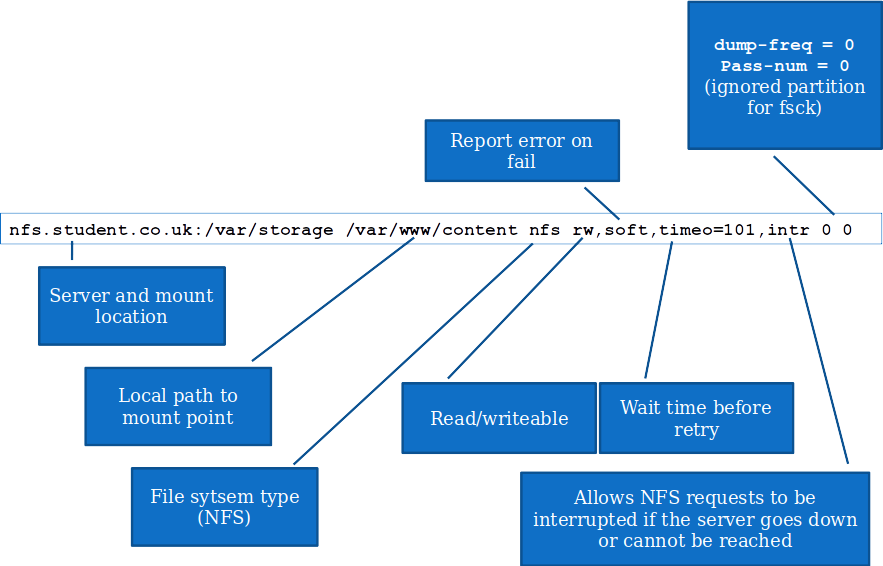
\includegraphics[width=1\linewidth]{fstab.png}
    \end{center}
  \end{figure}
\end{frame}

\begin{frame}[fragile]{Display currently mounted file systems}
  \begin{itemize}
    \item The \texttt{mount} command with no parameters will display the mount points of all current file systems.
  \end{itemize}
  \begin{tcolorbox}
    \lstset{
      basicstyle=\tiny\ttfamily,
    }
    \begin{lstlisting}
/dev/sda1 on / type ext4 (rw,errors=remount-ro)
proc on /proc type proc (rw,noexec,nosuid,nodev)
sysfs on /sys type sysfs (rw,noexec,nosuid,nodev)
fusectl on /sys/fs/fuse/connections type fusectl (rw)
none on /sys/kernel/debug type debugfs (rw)
none on /sys/kernel/security type securityfs (rw)
udev on /dev type devtmpfs (rw,mode=0755)
devpts on /dev/pts type devpts (rw,noexec,nosuid,gid=5,mode=0620)
tmpfs on /run type tmpfs (rw,noexec,nosuid,size=10%,mode=0755)
none on /run/lock type tmpfs (rw,noexec,nosuid,nodev,size=5242880)
none on /run/shm type tmpfs (rw,nosuid,nodev)
192.168.101.6:/home/student/test on /home/student/storage type nfs4 ...
(rw,addr=192.168.101.6,clientaddr=192.168.101.2)
    \end{lstlisting}
  \end{tcolorbox}
\end{frame}

\begin{frame}{Web content storage}
  \begin{figure}
    \begin{center}
      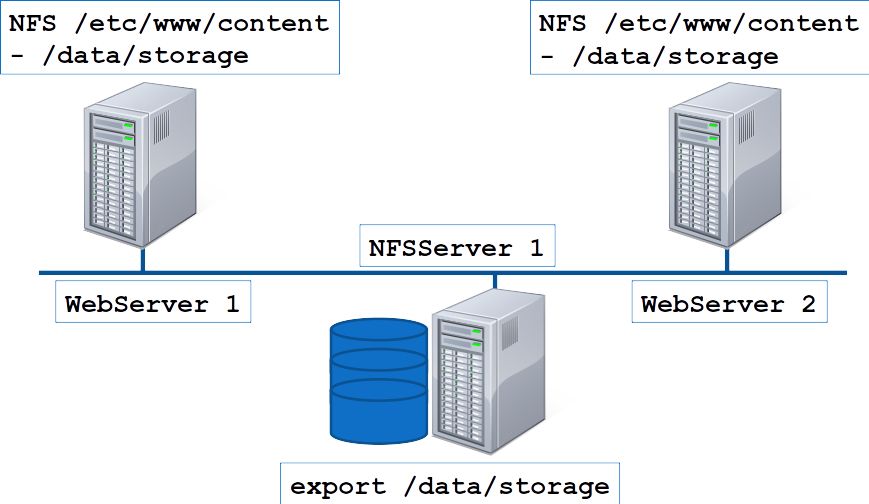
\includegraphics[width=1\linewidth]{webstorage.png}
    \end{center}
  \end{figure}
\end{frame}

\section{Scalability}
\subsection{Alternative Deployments}
\begin{frame}{Think Big! - \small{(Fancy a final year project?)}}
  \begin{figure}
    \begin{center}
      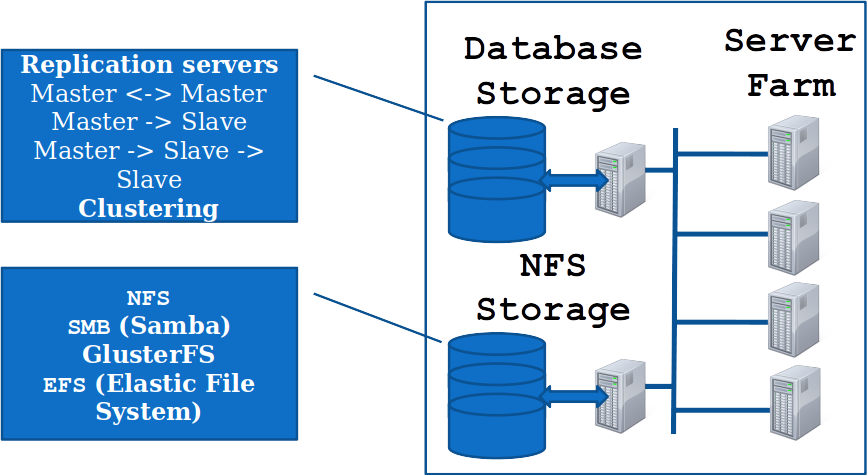
\includegraphics[width=1\linewidth]{Scalability.png}
    \end{center}
  \end{figure}
\end{frame}

\section*{Conclusion}
\begin{frame}{Conclusion}
  \begin{itemize}
    \item What is (Network) Content Storage and how is it used?
    \item What is \texttt{NFS}?
    \item How are \texttt{NFS} servers and clients configured?
    \item How does shared content storage relate to web services?
  \end{itemize}
\end{frame}

\end{document}


